\documentclass[zh]{nccuthesis}

\usepackage{times}
\usepackage{verbatim}
\usepackage{color}
\usepackage{url}
\usepackage{graphicx}
\usepackage{array}
\usepackage{pdfpages} % include outside .pdf
\usepackage{wallpaper} % watermark
% for table generate
\usepackage{mathtools}
\usepackage{amsmath}
\usepackage{amssymb}
\usepackage{booktabs}
\usepackage{adjustbox}

\usepackage{multirow}
\usepackage{multicol}
\usepackage{subfigure}

% Format the refs
\usepackage[sort,comma]{natbib}
\usepackage[hidelinks]{hyperref}

% For the tree
\usepackage{tikz}
\usepackage{tikz-qtree}

% For barchart
\usepackage{pgfplots}

% Using the tex-text mapping for ligatures etc.
\defaultfontfeatures{Mapping=tex-text}

% Set the default fonts
\setmainfont{Times New Roman}
\setCJKmainfont{TW-Kai}

% Your information goes here
% author: Ray Lu
% ----------------------------------------------------------------------------
% "THE CHOCOLATE-WARE LICENSE":
% Tz-Huan Huang originally wrote this file. As long as you retain this notice you
% can do whatever you want with this stuff. If we meet some day, and you think
% this stuff is worth it, you can buy me a chocolate in return Tz-Huan Huang
% ----------------------------------------------------------------------------


% 若需在封面加入英文資訊,可在下方第一個{}中進行修改,若是需要顯示學院名稱,僅須將%\college前的‘%’去除後再重新編譯即可。
%下方{}內資訊及為封面資訊設定,可自由進行修改,若需顯示英文資訊可至nccuthesisi.cls中查看相關說明。

% Syntax: \var{English}{Chinese}
\university{National Chengchi University (NCCU)}{國立政治大學}
%\college{College of Social Science}{社會科學院}
\institute{Department of Economics}{寵物溝通學系碩士班}
\title{If a dog encounter a police dog does it treat this as we see the police? }{狗狗看到警犬是否會覺得他看到警察了?}
\author{Yo-ro Huang}{黃有肉\ 撰}
\studentid{188258099}
\advisor{Piao Huang, Ph.D. \\}{黃裕誠\ 博士 \\}
\defenseyear{2022}{111}
\defensemonth{June}{6}
\defenseday{23}

\pgfplotsset{compat=1.14}
\begin{document}

% 政大論文浮水印
% 政大論文浮水印
% \CenterWallPaper{0.174}{pdfs/watermark.pdf}
% \setlength{\wpXoffset}{6.1725cm}
% \setlength{\wpYoffset}{10.5225cm}

\CenterWallPaper{}{pdfs/watermark.pdf}
\setlength{\wpXoffset}{0pt}
\setlength{\wpYoffset}{0pt}

\hypersetup{pageanchor=false}


\frontmatter
\pagenumbering{gobble}
\makecover

\clearpages
\setcounter{page}{1}
\hypersetup{pageanchor=true}
\pagenumbering{roman}
\phantomsection

% generate certification
% \makecertification
% or include scanned pdf


\begin{acknowledgementszh}
時光荏苒,感恩感恩,時光荏苒,感恩感恩,時光荏苒,感恩感恩,時光荏苒,感恩感恩,時光荏苒,感恩感恩,時光荏苒,感恩感恩,時光荏苒,感恩感恩,時光荏苒,感恩感恩,時光荏苒,感恩感恩,時光荏苒,感恩感恩,時光荏苒,感恩感恩,時光荏苒,感恩感恩,時光荏苒,感恩感恩,時光荏苒,感恩感恩,時光荏苒,感恩感恩,時光荏苒,感恩感恩,時光荏苒,感恩感恩,時光荏苒,感恩感恩,時光荏苒,感恩感恩,時光荏苒,感恩感恩,時光荏苒,感恩感恩,時光荏苒,感恩感恩,時光荏苒,感恩感恩,時光荏苒,感恩感恩,時光荏苒,感恩感恩,時光荏苒,感恩感恩,時光荏苒,感恩感恩,時光荏苒,感恩感恩,時光荏苒,感恩感恩,時光荏苒,感恩感恩,時光荏苒,感恩感恩,時光荏苒,感恩感恩,時光荏苒,感恩感恩,時光荏苒,感恩感恩,時光荏苒,感恩感恩,時光荏苒,感恩感恩,時光荏苒,感恩感恩,時光荏苒,感恩感恩。\par


\begin{flushright}
黃有肉  \qquad 謹致於\par

政治大學寵物溝通研究所\par

中華民國一一一年六月\par

\end{flushright}

\end{acknowledgementszh}



%%中英文摘要皆寫於本檔案即可abstractzh下方撰寫中文摘要 abstracten下方撰寫英文摘要。





\begin{abstractzh}
中文行距測試,中文行距測試,中文行距測試,中文行距測試,中文行距測試,中文行距測試,中文行距測試,中文行距測試,中文行距測試,中文行距測試,中文行距測試,中文行距測試,中文行距測試,中文行距測試,中文行距測試,中文行距測試,中文行距測試,中文行距測試,中文行距測試,中文行距測試,中文行距測試,中文行距測試,中文行距測試,中文行距測試,中文行距測試,中文行距測試,中文行距測試,中文行距測試,中文行距測試,中文行距測試,中文行距測試,中文行距測試,中文行距測試,中文行距測試,中文行距測試,中文行距測試,中文行距測試,中文行距測試,中文行距測試,中文行距測試,中文行距測試,中文行距測試,中文行距測試,中文行距測試,中文行距測試,中文行距測試,中文行距測試,中文行距測試,中文行距測試,中文行距測試,中文行距測試,中文行距測試,中文行距測試,中文行距測試,中文行距測試,中文行距測試,中文行距測試,中文行距測試,中文行距測試,中文行距測試,中文行距測試,中文行距測試,中文行距測試。


~\\
\noindent
關鍵字:狗狗、可愛、警犬、警察
\end{abstractzh}

\begin{abstracten}
\begin{small}
This is the English ident test.This is the English ident test.This is the English ident test.This is the English ident test.This is the English ident test.This is the English ident test.This is the English ident test.This is the English ident test.This is the English ident test.This is the English ident test.This is the English ident test.This is the English ident test.This is the English ident test.This is the English ident test.This is the English ident test.This is the English ident test.This is the English ident test.This is the English ident test.This is the English ident test.This is the English ident test.This is the English ident test.This is the English ident test.This is the English ident test.This is the English ident test.This is the English ident test.This is the English ident test.This is the English ident test.This is the English ident test. 

~\\
\noindent
Keywords: Dog, Cute, Police Dog, Police
\end{small}
\end{abstracten}




\newenvironment{changemargin}[2]{%
\begin{list}{}{

\setlength{\topmargin}{#1}
\setlength{\footskip}{#2}
}%
\item[]}{\end{list}}
% Table of Content
\clearpages
\begin{changemargin}{-2cm}{2.5cm}
\begin{small}
\tableofcontents
\end{small}
\end{changemargin}
% List of Figures

\clearpages
\listoffigures
% List of Tables
\clearpages
\listoftables

\mainmatter

% Your thesis goes here
\chapter{緒論}  %可更改{}中的文字來更改大標題名稱
\label{c:intro}


%若想新增新的節可用\section{}來加入
%段落結束後可使用\par來結束段落
\section{插入公式}

狗狗可愛貓貓更可愛,狗狗可愛貓貓更可愛,狗狗可愛貓貓更可愛,狗狗可愛貓貓更可愛,狗狗可愛貓貓更可愛,狗狗可愛貓貓更可愛,狗狗可愛貓貓更可愛,狗狗可愛貓貓更可愛,狗狗可愛貓貓更可愛,狗狗可愛貓貓更可愛,狗狗可愛貓貓更可愛,狗狗可愛貓貓更可愛,狗狗可愛貓貓更可愛,狗狗可愛貓貓更可愛,狗狗可愛貓貓更可愛,狗狗可愛貓貓更可愛,狗狗可愛貓貓更可愛,狗狗可愛貓貓更可愛,狗狗可愛貓貓更可愛,狗狗可愛貓貓更可愛,狗狗可愛貓貓更可愛,狗狗可愛貓貓更可愛,狗狗可愛貓貓更可愛,狗狗可愛貓貓更可愛,狗狗可愛貓貓更可愛,狗狗可愛貓貓更可愛,狗狗可愛貓貓更可愛,狗狗可愛貓貓更可愛,狗狗可愛貓貓更可愛,狗狗可愛貓貓更可愛,如下式$1.1$。\par

%%可以使用以下格式在文章中插入公式,所插入的公式會自行依照章節編號,正文中引用請使用$X.X$來引用,範例如上

\begin{equation}
h_{t} = c + \sum_{i=1}^{q}\alpha_{i} \epsilon^2_{t-1} + \sum_{j=1}^{p}\beta_{j} h_{t-1} \quad; \mbox{where} \quad v_{t}\overset{\mathrm{iid}}{\sim}(0,1)
\end{equation}



狗狗可愛貓貓更可愛,狗狗可愛貓貓更可愛,狗狗可愛貓貓更可愛,狗狗可愛貓貓更可愛,狗狗可愛貓貓更可愛,狗狗可愛貓貓更可愛,狗狗可愛貓貓更可愛,狗狗可愛貓貓更可愛,狗狗可愛貓貓更可愛,狗狗可愛貓貓更可愛,狗狗可愛貓貓更可愛,狗狗可愛貓貓更可愛,狗狗可愛貓貓更可愛,狗狗可愛貓貓更可愛,狗狗可愛貓貓更可愛,狗狗可愛貓貓更可愛,狗狗可愛貓貓更可愛,狗狗可愛貓貓更可愛,狗狗可愛貓貓更可愛,狗狗可愛貓貓更可愛,狗狗可愛貓貓更可愛,狗狗可愛貓貓更可愛,狗狗可愛貓貓更可愛,狗狗可愛貓貓更可愛,狗狗可愛貓貓更可愛,狗狗可愛貓貓更可愛,狗狗可愛貓貓更可愛。

\section{研究方法}

狗狗可愛貓貓更可愛,狗狗可愛貓貓更可愛,狗狗可愛貓貓更可愛,狗狗可愛貓貓更可愛,狗狗可愛貓貓更可愛,狗狗可愛貓貓更可愛,狗狗可愛貓貓更可愛,狗狗可愛貓貓更可愛,狗狗可愛貓貓更可愛,狗狗可愛貓貓更可愛,狗狗可愛貓貓更可愛,狗狗可愛貓貓更可愛,狗狗可愛貓貓更可愛,狗狗可愛貓貓更可愛,狗狗可愛貓貓更可愛,狗狗可愛貓貓更可愛,狗狗可愛貓貓更可愛,狗狗可愛貓貓更可愛,狗狗可愛貓貓更可愛,狗狗可愛貓貓更可愛,狗狗可愛貓貓更可愛,狗狗可愛貓貓更可愛,狗狗可愛貓貓更可愛,狗狗可愛貓貓更可愛,狗狗可愛貓貓更可愛,狗狗可愛貓貓更可愛,狗狗可愛貓貓更可愛。
\chapter{文獻回顧}

\section{插入圖片範例}

我是有肉,我是有肉,我是有肉,我是有肉,我是有肉,我是有肉,我是有肉,我是有肉,我是有肉,我是有肉,我是有肉,我是有肉,我是有肉,我是有肉,我是有肉,我是有肉,我是有肉,我是有肉,我是有肉,我是有肉,我是有肉,我是有肉,我是有肉,我是有肉,我是有肉,我是有肉,我是有肉,我是有肉,我是有肉,我是有肉,我是有肉,我是有肉,我是有肉,我是有肉。%%%之後若需加入新圖片僅需依照本檔案格式來創建即可,在本文中插入圖片的方式可參考chapters中文獻回顧檔案的範例。

%-------------------------------------------------------------


\begin{figure}[!htbp]

\centering


%上傳完成後至此資料夾創建一個新的檔案
%下面這行的最後一個{}加入image 中的圖片路徑
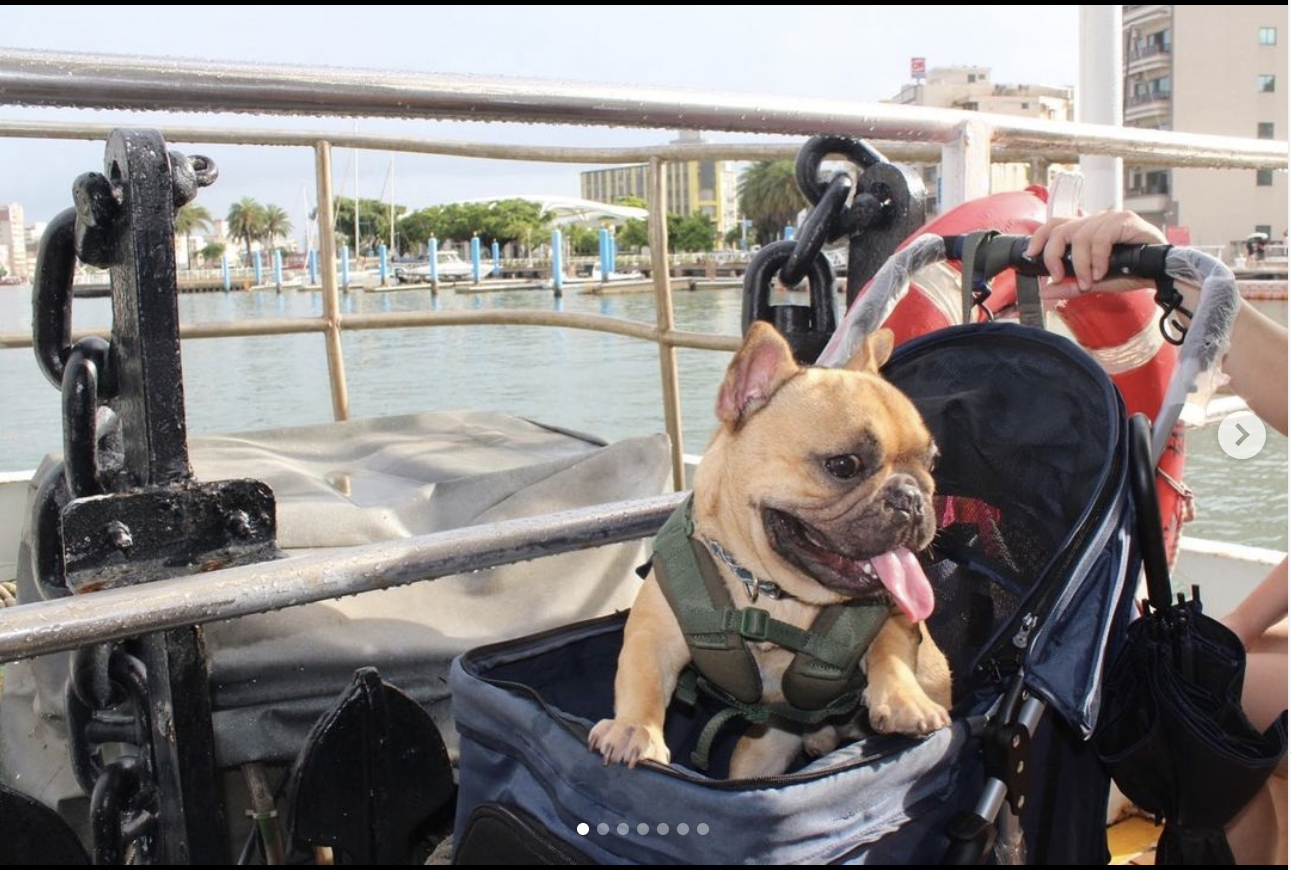
\includegraphics[width=1\textwidth]{images/yolo.png}

%下面這行書入圖片標題即可
\caption{有肉可愛}



\label{i:flow chart}
\end{figure}




我是有肉,我是有肉,我是有肉,我是有肉,我是有肉,我是有肉,我是有肉,我是有肉,我是有肉,我是有肉,我是有肉,我是有肉,我是有肉,我是有肉,我是有肉,我是有肉,我是有肉,我是有肉,我是有肉,我是有肉,我是有肉,我是有肉,我是有肉,我是有肉,我是有肉,我是有肉,我是有肉,我是有肉,我是有肉,我是有肉,我是有肉,我是有肉,我是有肉,我是有肉,我是有肉。/par



%%如上只需使用\input{圖片路徑}即可插入圖片。
%%所插入的圖片會自動依照章節編入圖目錄中,無需再進行更動。
















































\chapter{研究方法}

\section{表格範例}
我的體重表,我的體重表,我的體重表,我的體重表,我的體重表,我的體重表,我的體重表,我的體重表,我的體重表,我的體重表,我的體重表,我的體重表,我的體重表,我的體重表,我的體重表,我的體重表,我的體重表,我的體重表,我的體重表,我的體重表,我的體重表,我的體重表,我的體重表,我的體重表,我的體重表,我的體重表,我的體重表,我的體重表,我的體重表,我的體重表,我的體重表,我的體重表,我的體重表,我的體重表,我的體重表,我的體重表,我的體重表,我的體重表,我的體重表~\ref{3-1}。

%%%之後若需製作新表格僅需依照本檔案格式來創建即可,在本文中插入表格的方式可參考chapters中研究方法檔案的範例。
%------------------------------------------------------------

\begin{table}[htbp]

%%更改下一行{}中的文字即可更改表格名稱
\caption{狗狗視力檢定}
\begin{center}% used the environment to augment the vertical space
% between the caption and the table

%務必在下方{}中加上表格章節編號
\label{3-1}
\begin{adjustbox}{max width=1\textwidth}

%以下為範例表格,若需要其他種格式的表格可以自行搜尋Latex語法製作表格的方式將以下16行到32行代換掉即可。
\begin{tabular}{l c c c c c c  p{0cm} }
\toprule



& \multicolumn{2}{c}{A}& \multicolumn{2}{c}{b} & \multicolumn{2}{c}{d} \\ 
\cmidrule(lr){2-7}
& Statistic &  P-value & Statistic &  P-value & Statistic &  P-value  \\
\midrule
Realized Volatility &-11.98*** &0.00 &0.00208 &0.253 &-36.836*** &0.00 \\
Bitcoin Return &-18.13*** &0.00 &0.365 &0.089 &-40.512*** &0.00 \\
        
\bottomrule

\end{tabular}
\end{adjustbox}
\end{center}



\end{table}



我的體重表,我的體重表,我的體重表,我的體重表,我的體重表,我的體重表,我的體重表,我的體重表,我的體重表,我的體重表,我的體重表,我的體重表,我的體重表,我的體重表,我的體重表,我的體重表,我的體重表,我的體重表,我的體重表,我的體重表,我的體重表,我的體重表,我的體重表,我的體重表,我的體重表,我的體重表,我的體重表,我的體重表,我的體重表,我的體重表。


%%如上只需使用\input{表格路徑}即可插入表格。
%%所插入的表格會自動依照章節編入表目錄中,無需再進行更動。
%%若需在文章中引用表格可採用~\ref{表格章節編號}。
\chapter{實證結果}
\label{c:implement}

\section{插入小節及編號}

小節獵人測試,小節獵人測試,小節獵人測試,小節獵人測試,小節獵人測試,小節獵人測試,小節獵人測試,小節獵人測試,小節獵人測試,小節獵人測試,小節獵人測試,小節獵人測試,小節獵人測試,小節獵人測試,小節獵人測試,小節獵人測試,小節獵人測試,小節獵人測試,小節獵人測試,小節獵人測試,小節獵人測試,小節獵人測試,小節獵人測試,小節獵人測試,小節獵人測試,小節獵人測試,小節獵人測試,小節獵人測試,小節獵人測試,小節獵人測試,小節獵人測試,小節獵人測試,小節獵人測試,小節獵人測試,小節獵人測試,小節獵人測試,小節獵人測試。




\begin{itemize}
\begin{large}
\item[一、]
警犬  
\end{large}
\end{itemize}
分不出來,分不出來,分不出來,分不出來,分不出來,分不出來,分不出來,分不出來,分不出來,分不出來,分不出來,分不出來,分不出來,分不出來,分不出來,分不出來,分不出來,分不出來,分不出來,分不出來,分不出來,分不出來,分不出來,分不出來,分不出來,分不出來,分不出來,分不出來,分不出來,分不出來,分不出來,分不出來,分不出來。

\begin{itemize}
\begin{large}
\item[二、]
警察
\end{large}
\end{itemize}


分得出來,分得出來,分得出來,分得出來,分得出來,分得出來,分得出來,分得出來,分得出來,分得出來,分得出來,分得出來,分得出來,分得出來,分得出來,分得出來,分得出來,分得出來,分得出來,分得出來,分得出來,分得出來,分得出來,分得出來,分得出來,分得出來,分得出來,分得出來,分得出來。

\begin{itemize}
\item[1.]
騙我?
\end{itemize}

真的嗎?真的嗎?真的嗎?真的嗎?真的嗎?真的嗎?真的嗎?真的嗎?真的嗎?真的嗎?真的嗎?真的嗎?真的嗎?真的嗎?真的嗎?真的嗎?真的嗎?真的嗎?真的嗎?真的嗎?真的嗎?真的嗎?真的嗎?真的嗎?真的嗎?真的嗎?真的嗎?真的嗎?真的嗎?真的嗎?真的嗎?真的嗎?真的嗎?真的嗎?真的嗎?真的嗎?真的嗎?真的嗎?



\begin{itemize}
\item[2.]
真的
\end{itemize}
真的嗎?真的嗎?真的嗎?真的嗎?真的嗎?真的嗎?真的嗎?真的嗎?真的嗎?真的嗎?真的嗎?真的嗎?真的嗎?真的嗎?真的嗎?真的嗎?真的嗎?真的嗎?真的嗎?真的嗎?真的嗎?真的嗎?真的嗎?真的嗎?真的嗎?真的嗎?真的嗎?真的嗎?真的嗎?真的嗎?真的嗎?真的嗎?真的嗎?


\begin{itemize}
\item[3.]
警犬對狗來說就是警察
\end{itemize}


真的嗎?真的嗎?真的嗎?真的嗎?真的嗎?真的嗎?真的嗎?真的嗎?真的嗎?真的嗎?真的嗎?真的嗎?真的嗎?真的嗎?真的嗎?真的嗎?真的嗎?真的嗎?真的嗎?真的嗎?真的嗎?真的嗎?真的嗎?真的嗎?真的嗎?真的嗎?真的嗎?真的嗎?真的嗎?真的嗎?真的嗎?真的嗎?真的嗎?真的嗎?真的嗎?真的嗎?真的嗎?真的嗎?真的嗎?真的嗎?
\chapter{結論與建議}
\label{c:experiment}

\section{註腳範例}
%使用\footnote{}可以插入註腳

狗狗看不出顏色,所以看到警犬跟警察其實分不出來。狗狗看不出顏色,所以看到警犬跟警察其實分不出來。狗狗看不出顏色,所以看到警犬跟警察其實分不出來。狗狗看不出顏色,所以看到警犬跟警察其實分不出來。狗狗看不出顏色,所以看到警犬跟警察其實分不出來。狗狗看不出顏色,所以看到警犬跟警察其實分不出來。狗狗看不出顏色,所以看到警犬跟警察其實分不出來。狗狗看不出顏色,所以看到警犬跟警察其實分不出來。狗狗看不出顏色,所以看到警犬跟警察其實分不出來。狗狗看不出顏色,所以看到警犬跟警察其實分不出來。狗狗看不出顏色,所以看到警犬跟警察其實分不出來。狗狗看不出顏色,所以看到警犬跟警察其實分不出來。狗狗看不出顏色,所以看到警犬跟警察其實分不出來。狗狗看不出顏色,所以看到警犬跟警察其實分不出來。狗狗看不出顏色,所以看到警犬跟警察其實分不出來。狗狗看不出顏色,所以看到警犬跟警察其實分不出來。狗狗看不出顏色,所以看到警犬跟警察其實分不出來。\footnote{引注自:Discovery}


\section{參考文獻引用方法}
%首先需要獲取所需引用的參考文獻的APA檔,可以自行google或參考GitHub repo的README。

%先將所參考文獻的APA檔寫至thesis.bib中,即可在正文中使用\cite{}來飲用參考文獻。

根據\cite{slabbert1999early}的研究中所提出的觀點,狗可能真的可以分辨出警犬跟一般犬(並沒有!)。


\@startappendix


\backmatter

\clearpages
\phantomsection
\addcontentsline{toc}{chapter}{\bibname}
\bibliographystyle{apalike}
% Your bibliography goes here
\bibliography{thesis}

\end{document}
